\chapter{Uvod} \label{uvod}

Skozi celotno zgodovino so si ljudje želeli olajšati fizična dela na različne načine. Ponavljajoča dela je olajšala uporaba pogonov. Električni pogoni so delovne procese optimizirali. Za točnejše delovanje so se razvili različni načini krmiljenja. Z novimi načini krmiljenja, so se pojavile tudi potrebe po merjenju novih količin. V zadnjih desetletjih, je pri krmiljenuju, potrebna informacija o trenutnem položaju pogona.

Trenutni položaj merijo dajalniki pomika ali zasuka\cite{uporabaSenzorjev}. Pri rotacijskih dajalnikih ločimo dajalnike, ki merijo zasuk na koncu osi (angl.: on axis) in dajalnike, ki merijo zasuk na osi (angl.: through hole). Možna delitev rotacijskih dajalnikov je tudi na eno-obratne (angl.: single-turn) in več-obratne (angl.: multi-turn). Eno-obratni rotacijski dajalniki podajo položaj znotraj enega obrata, medtem ko več-obratni štejejo tudi število polnih obratov. Dajalnike položaja delimo tudi glede na uporabljeni princip zaznavanja fizikalne
spremembe, torej glede na uporabljeno tehnologijo. Poznamo magnetne, optične,
induktivne in druge\cite{killer}.

Pri magnetnem principu senzor dajalnika zaznava spremembo jakosti in smeri
magnetnega polja. 
Magnetno polje se ustvari z aktuatorjem radialno polariziranega magneta. Meri se s Hallovimi sondami ali AMR senzorji. Iz zajetega polja sledi izračun dejanskega položaja. Dajalnik položaja, ki pretvarja merjeno magnetno polje v informacijo o položaju imenujemo enkoder\cite{enkoder}.

Kot vsak merilni element, ima tudi magnetni enkoder napako. Napaka se lahko pojavi ob narobe merjenem magnetnem polju\cite{RLS3}. Napako lahko povzroči tudi napačno pomerjeno polje. To se zgodi ob nepravilni montaži enkoderja ali magnetnega aktuatorja na pogon. S poznavanjem vplivov nepravilne montaže na napako pomerjenega položaja, se napako lahko predvivi in odstrani.
Cilj naloge je analizirtai kako različne napake pri montaži, vplivajo na napako v signalih kota.
Želi se predstaviti čimbolj preprost model, ki bo dovolj točno opisal dogajanje ob prisotnosti napake in to prekontrolirati.


%V tej magistrski nalogi je predstavljen vpliv napačno merjenega magnetnega polja. Predstavljen je simulacijski model enkoderja, ter odvistnost napake na nepravilno montažo. Simulacije so primerjane z meritvami na enkoderju RM44\cite{RM44}.


\chapter{Senzor RM44}

Senzor RM44 je 13 bitni enkoder, primeren za merjenje zasuka in hitrosti elektromotorskega pogona\cite{RM44}.
Enkoder se nahaja v robustem ohišju, zato je primeren za delovanje v težkem industrijskem okolju. % , pritrjenega na konec rotirajoče osi pogonskega sklopa.
Obliko izhodnega podatka o zasuku, je prilagodljiva na sistem aplikacije v kateri bo uporabljen\cite{Ambrozic}. Izhod senzorja je lahko analogni, v obliki sinusa in cosinusa, inkrementalni \cite{inkrementalni} s signaloma A in B s katerih lahko izračunamo smer vrtenja ter signal Ri kateri določa referenčno točko. Izhod je lahko tudi digitalen preko komunikacijo SSI ali analogna napetost, ki se linearno spreminja med potencialom GND in Vdd v odvistnosti od kota zasuka. Senzor ima možnost nastavitev resolucije od 5 do 13 bitov \cite{RM44}\cite{AM8192}. Senzor na katerem so bile opravljene meritve je imel na voljo analogna signala sinus in kosinus. Točno ime senzorja je RM44AC0001S20F2E10, v delu bo poimenovan okrajšano RM44.

Ključni element senzorja je čip AM512. V čipu so Hallove sonde za meritev z-komponente gostote magnetnega pretoka. 

\begin{figure}[h]
	\centering
	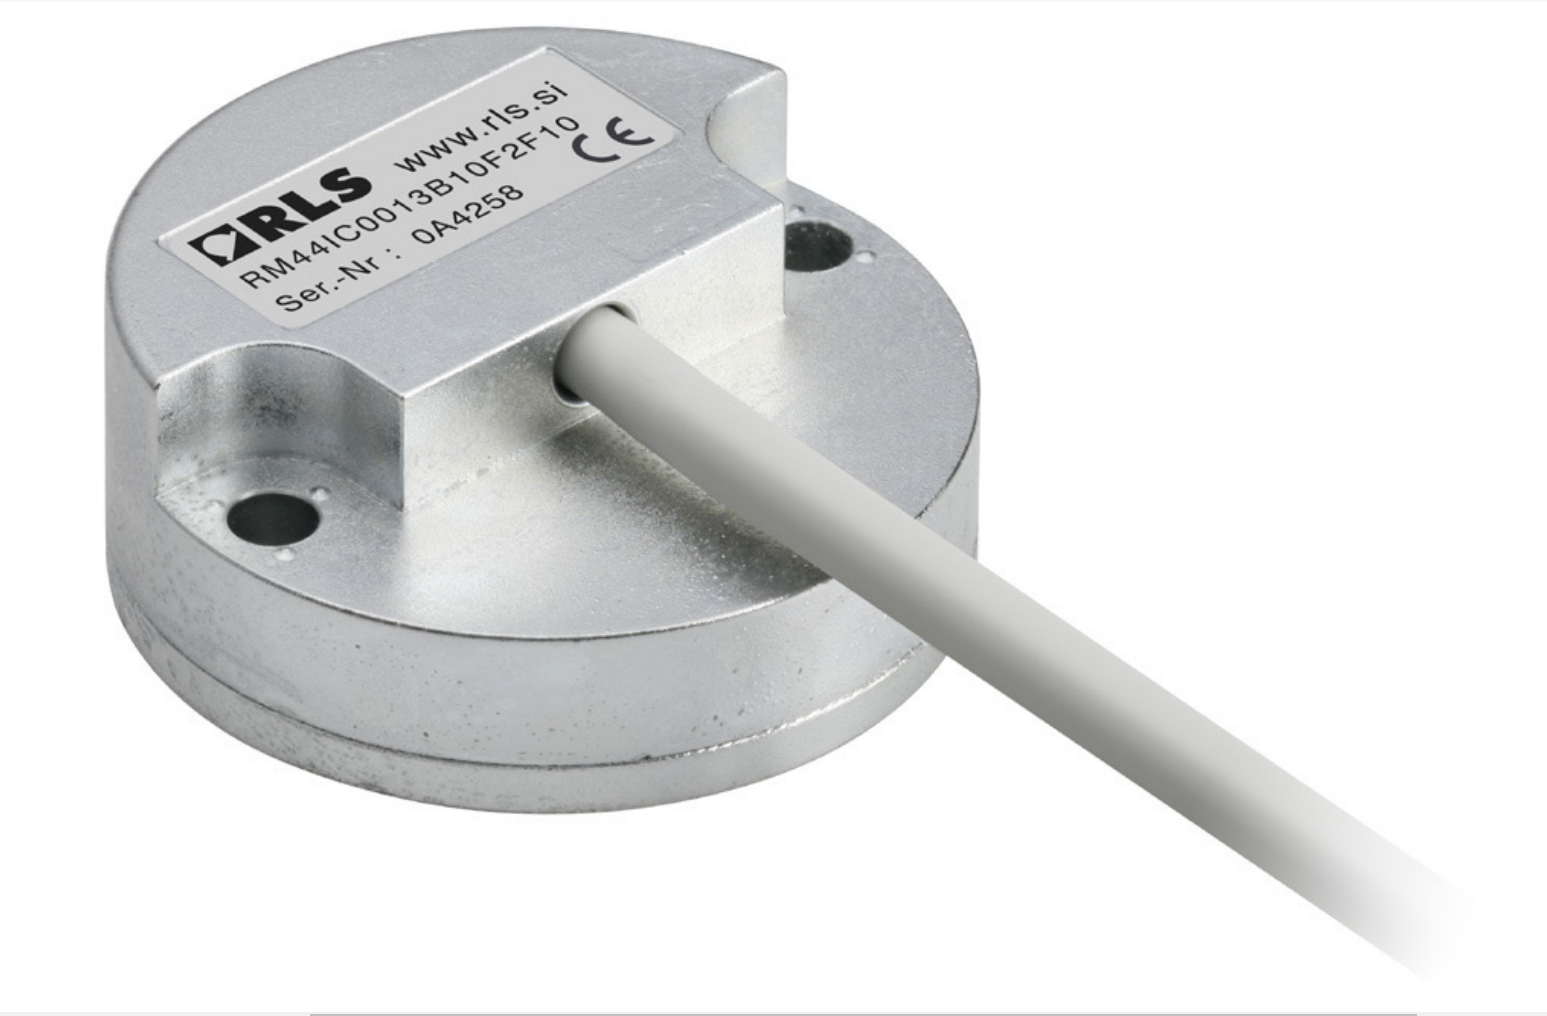
\includegraphics[width=0.8\columnwidth]{./Slike/senzorRM44.jpg}
	\caption{Senzor RM44}
	\label{RM44}
\end{figure}



\chapter{Zastavljena naloga}

Senzor RM44 mora biti za pravilno delovnanje in točnost izhodnega podatka pravilno montiran.% V podatkovnih listih je podana toleranca $\pm100\mathrm{\mu m}$. 

Magistrsko delo predstavlja vpliv nepravilno montiranega senzorja ali nepravilno montiranega magneta na napako. Kako nepravilna montaža vpliva na izhodna signala sinus in kosinus ter neposredno iz tega tudi na napako.
Različne literature so ocenjevale vpliv neidealnih analognih signalov za izračun kota\cite{osnova}\cite{RLS1}\cite{RLS2}. V delu je predstavljena odvisnost napake pri spremembi idealnih signalov sinus in kosinus na izračunan kot.

V začetku je bila opravljena  izpeljava kako se giblje magnet ali senzor v sistemu z nepravilno montažo\cite{ursic}. Opravil sem simulacije na linearno aproksimiranem magnetnem polju, ter na numerično izračunanem polju simuliranega realnega magneta.
Tehnologija senzorja RM44 je poslovna skrivnost, zato je bil postavljen lasten simulacijski model senzorja, s pričakovanji, da bo rezultat  slabši od končnih meritev.

Na tej točki bi bilo primerno definirati pojme, kateri se bodo uporabljali tekom izdelave dela.
Izmik senzorja bo med spreminjanja kota zasuka postavljen fiksno in se njegova lokacija nebo spreminjala na os vrtenja. Ta izmik je poimenovan statična ekscentričnost.
V nalogi bo preverjeno kako vpliva izmik magneta na točnost izhodnega podatka. Ob izmiku magneta iz osi vrtenja se pojavi opletanje magneta. Lokacija središča magneta se spreminja glede na določen zasuk magneta. Opletanje magneta je poimenovano dinamična ekscentričnost.














%
%Senzorji se delijo resolverje in enkoderje. Resolver ima unikatno oblikovan rotorski aktuator, kjer se med vretenjem zaradi posebne oblike, zračna reža spreminja sinusno. To ima za posledico istovrstno spreminjanje upornosti magnetnih poti fluksa med primarnimi in sekundarnimi glavami navitij ter nato induciranih napetosti \cite{Ursic}.
%
%
%delijo na absolutne ali inkrementalne merilnike. Inkrementalni nam sporočijo relativo spremembo zasuka, ob prehodu referenčne točke se lahko senzor šele inicializira in od takrat dalje je možen izračun dejsanskega zasuka. Primer takega senzorja je optični senzor zasuka.
%
%Absolutni dajalniki zasuka lahko neglede na dan zasuk razbere dejansko vrednost zasuka rotorja. Primera sta 
%
%Enkoder oz. rotacijski enkoder je naprava 